% A short document to try the plugin with: open it, then pick "Editor | PDF" in the view toggle.
\documentclass[11pt]{article}
\usepackage[margin=2.5cm]{geometry}
\usepackage{amsmath,amssymb}
\usepackage{booktabs}
\usepackage{tikz}
\usepackage[colorlinks,allcolors=blue!60!black]{hyperref}

\title{Heat Flow on a Thin Rod}
\author{A. Student}
\date{\today}

\begin{document}
\maketitle

\begin{abstract}
We derive the heat equation for a thin rod, solve it with separation of variables, and compare
the series solution with a finite-difference scheme. Figure~\ref{fig:rod} shows the set-up and
Table~\ref{tab:error} the error of each method.
\end{abstract}

\section{The heat equation}\label{sec:equation}
Let $u(x,t)$ be the temperature at position $x \in [0, L]$ and time $t \ge 0$. Conservation of
energy and Fourier's law give
\begin{equation}
  \frac{\partial u}{\partial t} = \alpha \, \frac{\partial^2 u}{\partial x^2},
  \qquad u(0,t) = u(L,t) = 0,
  \label{eq:heat}
\end{equation}
where $\alpha > 0$ is the thermal diffusivity~\cite{fourier1822,carslaw1959}.

\begin{figure}[ht]
  \centering
  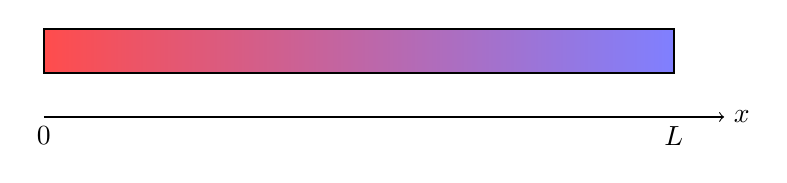
\begin{tikzpicture}[scale=1.6]
    \shade[left color=red!70, right color=blue!50] (0,0) rectangle (5,0.35);
    \draw[thick] (0,0) rectangle (5,0.35);
    \draw[->] (0,-0.35) -- (5.4,-0.35) node[right] {$x$};
    \node[below] at (0,-0.35) {$0$};
    \node[below] at (5,-0.35) {$L$};
  \end{tikzpicture}
  \caption{A rod held at zero temperature at both ends.}
  \label{fig:rod}
\end{figure}

\section{Separation of variables}\label{sec:series}
Writing $u(x,t) = X(x)\,T(t)$ in~\eqref{eq:heat} splits it into two ordinary equations, and the
boundary conditions leave the modes $X_n(x) = \sin(n\pi x / L)$. The solution is the series
\begin{equation}
  u(x,t) = \sum_{n=1}^{\infty} b_n \, e^{-\alpha (n\pi/L)^2 t} \sin\!\left(\frac{n\pi x}{L}\right),
  \qquad b_n = \frac{2}{L}\int_0^L u(x,0) \sin\!\left(\frac{n\pi x}{L}\right) dx .
  \label{eq:series}
\end{equation}
Higher modes decay quickly, so a few terms describe the rod well after a short time.

\section{A numerical check}\label{sec:numerics}
The explicit scheme $u_i^{k+1} = u_i^k + r\,(u_{i+1}^k - 2u_i^k + u_{i-1}^k)$ with
$r = \alpha\,\Delta t / \Delta x^2$ is stable for $r \le \tfrac12$~\cite{crank1947}.
Table~\ref{tab:error} compares it with ten terms of~\eqref{eq:series}.

\begin{table}[ht]
  \centering
  \caption{Largest error at $t = 0.1$ against the exact solution.}
  \label{tab:error}
  \begin{tabular}{lrr}
    \toprule
    Method & Grid points & Max.\ error \\
    \midrule
    Series, 10 terms & --- & $2.1 \times 10^{-6}$ \\
    Explicit, $r = 0.4$ & 51 & $3.8 \times 10^{-4}$ \\
    Explicit, $r = 0.4$ & 101 & $9.6 \times 10^{-5}$ \\
    \bottomrule
  \end{tabular}
\end{table}

Halving the grid spacing divides the error by about four, as the scheme is second order in
space (Section~\ref{sec:series} gives the exact values).

\bibliographystyle{plain}
\bibliography{refs}
\end{document}
